\chapter{VBF \hwwlnln analysis}\label{section:VBFanalysis}

This chapter is organized as follow. Section \ref{VBF:CommonSelection} provides ...

%Section \ref{subsec:data_trigger} discusses the triggers used, the trigger efficiencies and the gains of signals with the current setup.
\section{Common event selection}\label{VBF:CommonSelection}
...

\begin{itemize}
	\item Exactly two opposite charged and different flavor leptons ($e\mu+\mu e$)
	\item $\pTlead > 22$ \gev, $\pTsublead > 15$ \gev
	\item $\mll > 10$ \gev
\end{itemize}




\section{Construction of the VBF  phase space}\label{VBF:VBFSR}

\subsection{Experimental signature of VBF Higgs boson}\label{VBF:Signature}
The VBF production is characterized ... 




\subsection{Event selection for VBF-enriched phase space}\label{VBF:EventSelection}

After the common event selection ...

\begin{table}[!h]
	\centering
	\caption{Ranking of the BDT training variables \cite{ATLASComNote}.}
	\label{tab:ranking}
	\scalebox{0.8}{
		\vspace{0.3cm}
\begin{tabular}{ c | c  | c }
\hline
\hline
Ranking & Variable & Importance [\%]\\
\hline
1       & $\mathrm{m_{jj}}$            & 19\\
2       & $\mathrm {\Delta y_{jj}}$    & zz\\
3       & $\mathrm {m_{ll}}$           & xx\\
4       & $m_T$                        & yy\\
5       & lepton $\eta$ centrality     & zz\\
6       & $\mathrm{\Delta \phi_{ll}}$  & aa\\
7       & $\mathrm{\sum_{l,j} M_{lj}}$ & bb \\
8       & $\mathrm{p^{T}_{tot}}$       & cc \\
\hline
\hline
\end{tabular}

	}
\end{table}


%\begin{figure}[t]
%	\begin{minipage}{0.5\textwidth}
%		\centering
%		\includegraphics[width=0.9\linewidth, angle=-90]{Figures/VBFAnalysis/BDTInput/emme-CutVBFbVeto_2jet-Mll-lin}
%	\end{minipage}
%	\begin{minipage}{0.5\textwidth}
%		\centering
%		\includegraphics[width=0.9\linewidth, angle=-90]{Figures/VBFAnalysis/BDTInput/emme-CutVBFbVeto_2jet-DPhill-lin}
%	\end{minipage}
%		\begin{minipage}{0.5\textwidth}
%			\centering
%			\includegraphics[width=0.9\linewidth, angle=-90]{Figures/VBFAnalysis/BDTInput/emme-CutVBFbVeto_2jet-DYjj-lin}
%		\end{minipage}
%			\begin{minipage}{0.5\textwidth}
%				\centering
%				\includegraphics[width=0.9\linewidth, angle=-90]{Figures/VBFAnalysis/BDTInput/emme-CutVBFbVeto_2jet-Mjj-lin}
%			\end{minipage}
%		\caption{Distributions of BDT inputs $\mll$, $\dphill$, $\dyjj$ and $\mjj$ after VBF pre-selection. The VBF signal is scaled by a factor of 300 \cite{ATLASComNote}.}
%		\label{fig:BDTinput1}
%	\end{figure}

\begin{table}[!h]
	\centering
	\caption{ 
		Event yields in the VBF SR after fitting. Event yields in the highest BDT bin are also presented. The uncertainties include systematic and statistical uncertainties \cite{HWWRun2Paper}.}
	\label{tab:ggF_VBF_yields}
	\scalebox{0.8}{
		\begin{tabular}{lS[table-format=4.1,table-number-alignment=right]@{$\,\pm\,$}
                     S[table-format=3.2,table-number-alignment=left]
                     S[table-format=4.2,table-number-alignment=right]@{$\,\pm\,$}
                     S[table-format=3,table-number-alignment=left]
                     S[table-format=2,table-number-alignment=right]@{$\,\pm\,$}
%                     S[table-format=4.1,table-number-alignment=left]
%                     S[table-format=3.3,table-number-alignment=right]@{$\,\pm\,$}
%                     S[table-format=2,table-number-alignment=left]
                     }
  \dbline
  Process  & \multicolumn{5}{c}{\TwoJet VBF}  \tabularnewline
             &  \multicolumn{2}{c}{Inclusive} &\multicolumn{3}{c}{BDT: $[0.86,1.0]$}\tabularnewline
  \sgline
  $H_{\mathrm{ggF}}$                   &  42   & 16 & 6   &  3   \tabularnewline
  $H_{\mathrm{VBF}}$                  &  xx   & yy & zz  &  xx   \tabularnewline
  \sgline                                               
  $WW$                                &  xx   & yy & zz  &  xx    \tabularnewline
  $VV$                           &  xx   & yy & zz  &  xx    \tabularnewline
  $t\bar{t}/Wt$                     &  xx   & yy & zz  &  xx     \tabularnewline
  Mis-Id                           &  xx   & yy & zz  &  xx    \tabularnewline
  $Z/\gamma^{*}$                &  xx   & yy & zz  &  xx     \tabularnewline
  \sgline
  Total                         &  xx   & yy & zz  &  xx    \tabularnewline
  Observed   &  \multicolumn{2}{l}{2164}  & \multicolumn{2}{l}{\quad60}  \tabularnewline
  \dbline
  \end{tabular}
 
	}
\end{table}


\begin{figure}[!h]
\centering
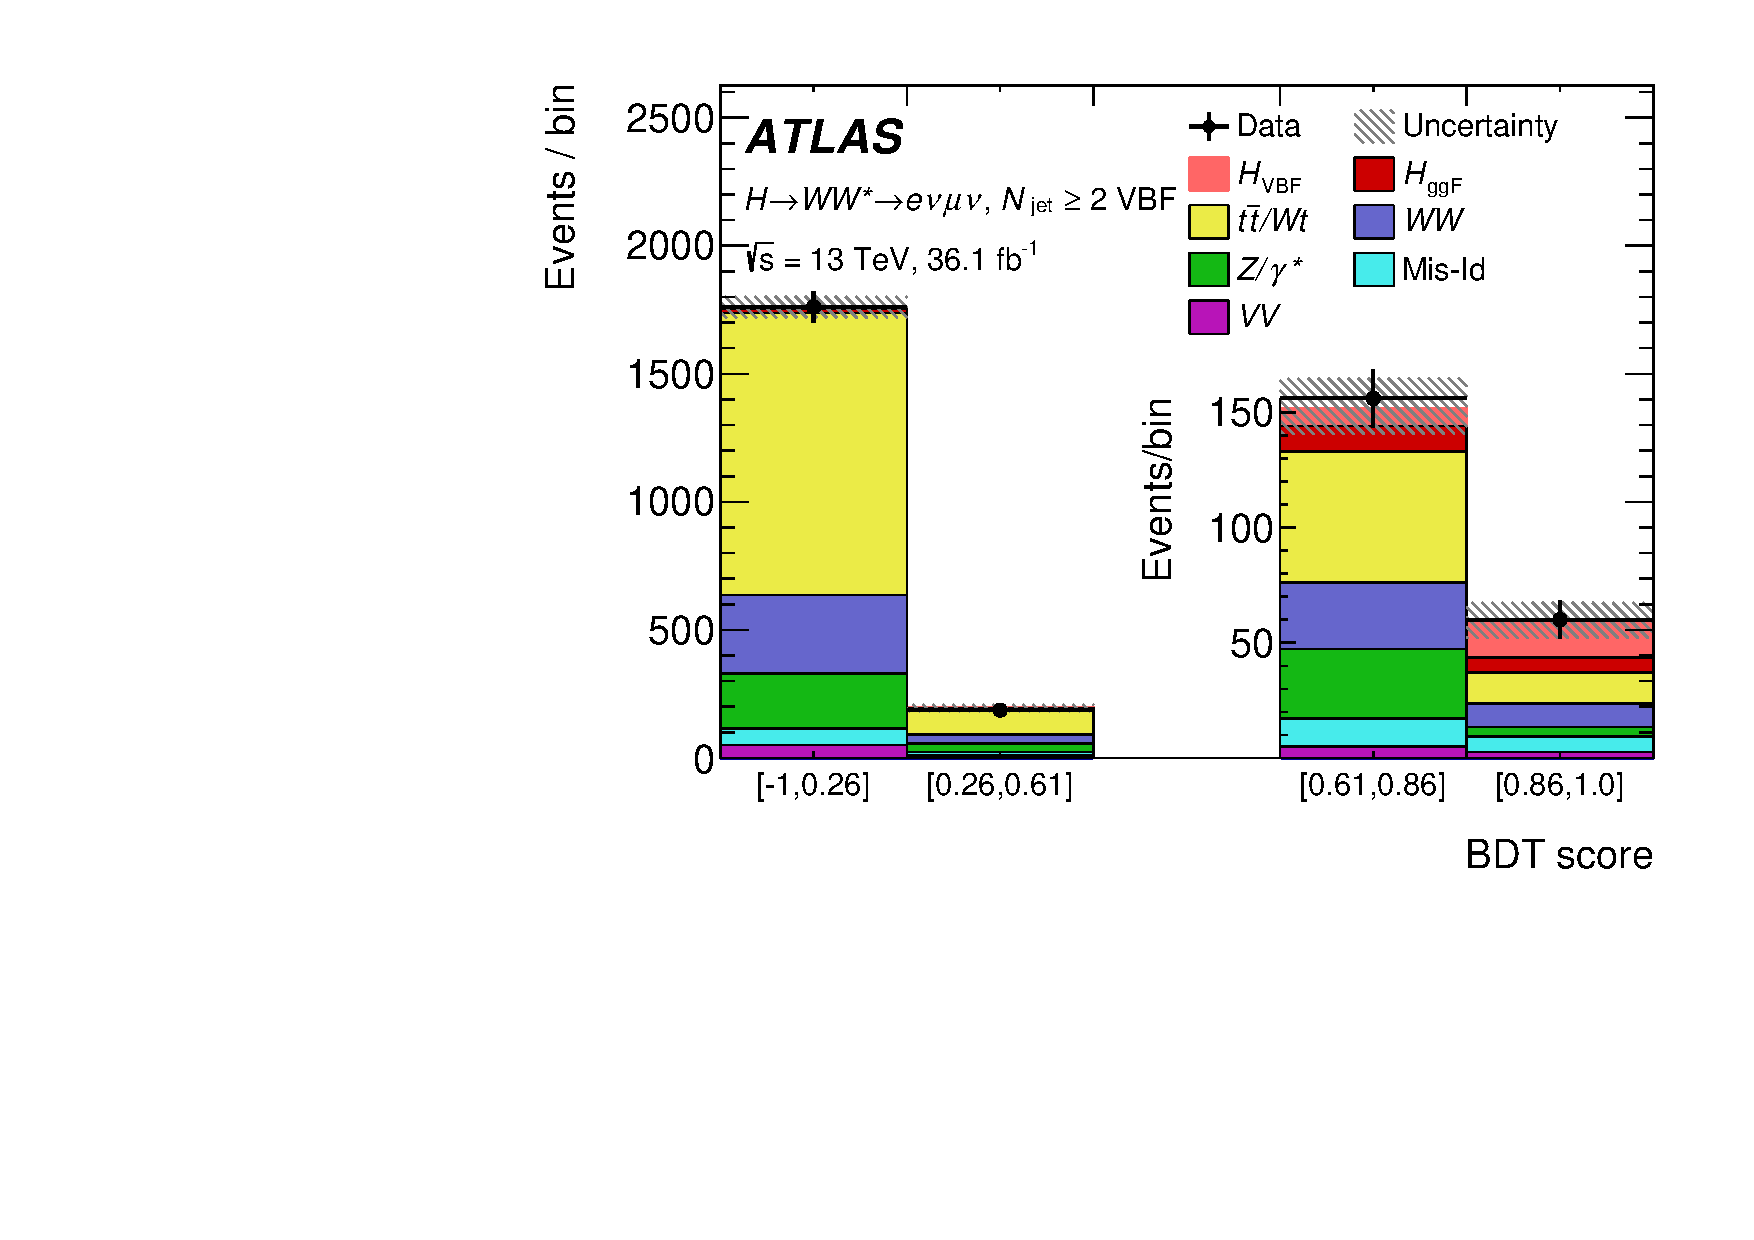
\includegraphics[width=0.45\linewidth, angle=-90]{Figures/VBFAnalysis/BDT_newStyle_V03}
\caption{Distribution of BDT scores in the VBF SR after fitting is shown. The hatched error band shows the total uncertainty of signal and background MC prediction \cite{HWWRun2Paper}.}
\label{fig:BDT_newStyle_V03}
\end{figure}

\section{Results of VBF analysis in Run-2}\label{VBF:Results}
The signal strength $\mu$ is the ratio of the measured signal yields to the signal yields predicted by the SM. The signal strength for VBF analysis in our final publication \cite{HWWRun2Paper} is shown below:

\begin{equation}
\mu_{\mathrm{VBF}} =  0.62^{+0.29}_{-0.27} (\mathrm{stat.})^{+0.12}_{-0.13} (\mathrm{theo~ syst.})\pm 0.15(\mathrm{exp~ syst.}) = 0.62^{+0.36}_{-0.35}.
\end{equation}\label{eqn:SignalStrength}

